% SMA-1 Methods figure -- Architecture / two-stage retrieval pipeline.
% Stage 1 (Load & register): loader -> normalized graph -> mount/case builder -> registry/router.
% Stage 2 (Match & decide): encode -> MAC -> FAC -> surprisal scorer -> {cite, abstain, novelty}.
% Conceptual / schematic only. NO numbers, accuracies, bars. Caption supplied by manuscript.
\documentclass[border=4pt]{standalone}
\usepackage{amsmath}
\usepackage{amssymb}
\usepackage{pifont}
\usepackage{fontspec}
\setsansfont{Arimo}
\renewcommand{\familydefault}{\sfdefault}
\usepackage{tikz}
\usetikzlibrary{arrows.meta,positioning,calc,fit,backgrounds,shapes.geometric,shapes.multipart,decorations.pathreplacing}

\definecolor{ink}{HTML}{1A1C1E}
\definecolor{ink7}{HTML}{3D4248}
\definecolor{ink5}{HTML}{6B7177}
\definecolor{ink4}{HTML}{8A9097}
\definecolor{ink3}{HTML}{B4B9BE}
\definecolor{ink2}{HTML}{D6D9DC}
\definecolor{ink1}{HTML}{EAECEE}
\definecolor{ink05}{HTML}{F4F5F6}
\definecolor{teal}{HTML}{3F8A83}
\definecolor{teal2}{HTML}{4FA89F}
\definecolor{tealtint}{HTML}{E6F0EF}
\definecolor{amber}{HTML}{C2883C}
\definecolor{ambertint}{HTML}{F6ECDD}
\definecolor{redf}{HTML}{C05A50}
\definecolor{redtint}{HTML}{F6E2E0}
\definecolor{greenk}{HTML}{3E9B63}
\definecolor{greentint}{HTML}{E2F0E8}
\definecolor{fo}{HTML}{5AA9C4}
\definecolor{ho}{HTML}{2E6B86}
\definecolor{vio}{HTML}{9B86C4}
\definecolor{viotint}{HTML}{ECE6F4}

% in-node font switches (no argument, so \\ stays at node level for align=center)
\newcommand{\BL}{\bfseries\fontsize{7}{8.4}\selectfont}
\newcommand{\NL}{\mdseries\fontsize{6}{7}\selectfont}

\begin{document}
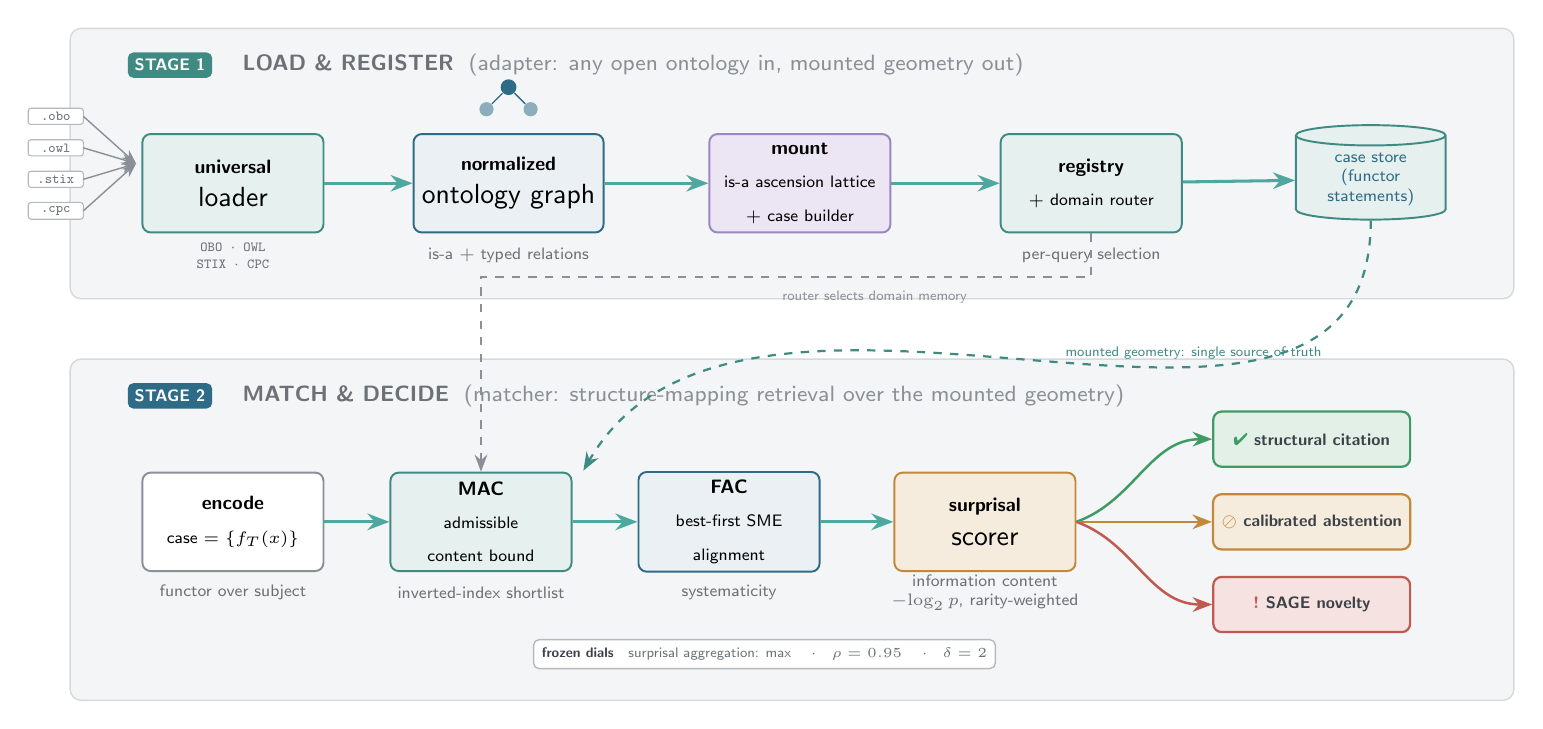
\begin{tikzpicture}[
  font=\sffamily,
  >=Stealth,
  stage/.style={font=\sffamily\bfseries\footnotesize, color=ink5},
  stagebadge/.style={font=\sffamily\bfseries\fontsize{6.4}{7}\selectfont, text=white},
  blab/.style={font=\sffamily\bfseries\fontsize{7}{8.4}\selectfont, text=ink, align=center},
  slab/.style={font=\sffamily\fontsize{5.8}{6.8}\selectfont, text=ink5, align=center},
  tinylab/.style={font=\sffamily\fontsize{5.2}{6}\selectfont, text=ink5, align=center},
  mono/.style={font=\ttfamily\fontsize{5.4}{6.4}\selectfont, text=ink5},
  % pipeline boxes
  pbox/.style={draw=ink3, fill=white, line width=0.7pt, rounded corners=3pt, align=center,
               minimum width=2.3cm, minimum height=1.25cm, inner sep=3pt},
  pteal/.style={pbox, draw=teal, fill=tealtint},
  pho/.style={pbox, draw=ho, fill=ho!10},
  pamber/.style={pbox, draw=amber, fill=ambertint},
  pvio/.style={pbox, draw=vio, fill=viotint},
  flow/.style={->, line width=1.0pt, color=ink5},
  flowt/.style={->, line width=1.1pt, color=teal2},
  outbox/.style={draw, line width=0.8pt, rounded corners=3pt, align=left, inner sep=3pt,
                 minimum width=2.5cm, minimum height=7mm, font=\sffamily\fontsize{6.2}{7.2}\selectfont},
  panelbg/.style={draw=ink2, line width=0.5pt, fill=ink05, rounded corners=4pt},
]

% ===================================================================
% Two horizontal lanes. Canvas approx 18.2 x 9.0
% Stage 1 row y ~ 6.6 ; Stage 2 row y ~ 2.4
% ===================================================================

% ---- stage background bands ----
\begin{scope}[on background layer]
  \node[panelbg, fit={(-0.1,5.35) (18.0,8.55)}] (S1bg) {};
  \node[panelbg, fit={(-0.1,0.25) (18.0,4.35)}] (S2bg) {};
\end{scope}

% =================== STAGE 1: LOAD & REGISTER ===================
\node[fill=teal, rounded corners=2pt, inner sep=2.5pt, stagebadge] at (1.05,8.2) {STAGE 1};
\node[stage, anchor=west] at (1.85,8.2) {LOAD \& REGISTER \;\textmd{\color{ink4}(adapter: any open ontology in, mounted geometry out)}};

% --- 1: universal loader ---
\node[pteal] (loader) at (1.85,6.7) {\BL universal\\loader};
\node[mono, align=center] at (1.85,5.78) {OBO $\cdot$ OWL\\STIX $\cdot$ CPC};
% small format chips feeding the loader
\foreach \fy/\ft in {7.55/.obo, 7.15/.owl, 6.75/.stix, 6.35/.cpc} {
  \node[draw=ink3, fill=white, rounded corners=1pt, font=\ttfamily\fontsize{4.6}{5.2}\selectfont, text=ink5, inner sep=1.4pt, minimum width=7mm] at (-0.4,\fy) {\ft};
  \draw[->, line width=0.5pt, color=ink4] (-0.05,\fy) -- (0.62,6.95);
}

% --- 2: normalized ontology graph ---
\node[pho] (norm) at (5.35,6.7) {\BL normalized\\ontology graph};
\node[slab] at (5.35,5.78) {is-a $+$ typed relations};
% mini is-a glyph above the box (not overlapping text)
\begin{scope}[shift={(5.35,7.78)}]
  \node[circle, fill=ho, minimum size=2.0mm, inner sep=0pt] (gr) at (0,0.14) {};
  \node[circle, fill=ho!55, minimum size=1.8mm, inner sep=0pt] (gl) at (-0.28,-0.14) {};
  \node[circle, fill=ho!55, minimum size=1.8mm, inner sep=0pt] (grr) at (0.28,-0.14) {};
  \draw[-, line width=0.5pt, color=ho] (gl)--(gr) (grr)--(gr);
\end{scope}

% --- 3: mount + case builder ---
\node[pvio] (mount) at (9.05,6.7) {\BL mount\\{\NL is-a ascension lattice}\\{\NL $+$ case builder}};

% --- 4: registry / router ---
\node[pteal] (reg) at (12.75,6.7) {\BL registry\\{\NL $+$ domain router}};
\node[slab] at (12.75,5.78) {per-query selection};

% --- case-store cylinder (write target) ---
\node[cylinder, shape border rotate=90, draw=teal, fill=tealtint, line width=0.7pt,
      aspect=0.22, minimum width=1.9cm, minimum height=1.2cm, inner sep=1pt,
      text=ho, font=\sffamily\fontsize{6}{7}\selectfont, align=center] (store) at (16.3,6.75) {case store\\(functor\\statements)};

% stage-1 flow
\draw[flowt] (loader) -- (norm);
\draw[flowt] (norm) -- (mount);
\draw[flowt] (mount) -- (reg);
\draw[flowt] (reg) -- (store);

% =================== STAGE 2: MATCH & DECIDE ===================
\node[fill=ho, rounded corners=2pt, inner sep=2.5pt, stagebadge] at (1.05,4.0) {STAGE 2};
\node[stage, anchor=west] at (1.85,4.0) {MATCH \& DECIDE \;\textmd{\color{ink4}(matcher: structure-mapping retrieval over the mounted geometry)}};

% --- query encode ---
\node[pbox, draw=ink4, fill=white] (qenc) at (1.85,2.4) {\BL encode\\{\NL case $=\{f_T(x)\}$}};
\node[slab] at (1.85,1.5) {functor over subject};

% --- MAC ---
\node[pteal] (mac) at (5.0,2.4) {\BL MAC\\{\NL admissible}\\{\NL content bound}};
\node[slab] at (5.0,1.5) {inverted-index shortlist};

% --- FAC ---
\node[pho] (fac) at (8.15,2.4) {\BL FAC\\{\NL best-first SME}\\{\NL alignment}};
\node[slab] at (8.15,1.5) {systematicity};

% --- surprisal scorer ---
\node[pamber] (score) at (11.4,2.4) {\BL surprisal\\scorer};
\node[slab, text width=2.6cm] at (11.4,1.5) {information content\\$-\!\log_2 p$, rarity-weighted};

% stage-2 flow
\draw[flowt] (qenc) -- (mac);
\draw[flowt] (mac) -- (fac);
\draw[flowt] (fac) -- (score);

% --- decision outputs (right) ---
\node[outbox, draw=greenk, fill=greentint, text=ink7] (cite) at (15.55,3.45)
     {\textbf{\textcolor{greenk}{\ding{52}} structural citation}};
\node[outbox, draw=amber, fill=ambertint, text=ink7] (abst) at (15.55,2.4)
     {\textbf{\textcolor{amber}{$\oslash$} calibrated abstention}};
\node[outbox, draw=redf, fill=redtint, text=ink7] (nov) at (15.55,1.35)
     {\textbf{\textcolor{redf}{$\boldsymbol{!}$} SAGE novelty}};

% branch from scorer to the three outcomes
\draw[->, line width=0.9pt, color=greenk] (score.east) to[out=20,in=180] (cite.west);
\draw[->, line width=0.9pt, color=amber]  (score.east) to[out=0,in=180]  (abst.west);
\draw[->, line width=0.9pt, color=redf]   (score.east) to[out=-20,in=180] (nov.west);

% --- read from case store down into the matcher (store feeds MAC/FAC) ---
\draw[->, line width=0.8pt, color=teal, dashed] (store.south) to[out=-90,in=60] (6.3,3.05);
\node[tinylab, text=teal, anchor=west] at (12.3,4.55) {mounted geometry: single source of truth};

% --- frozen dials annotation (light) ---
\node[draw=ink3, fill=white, rounded corners=2pt, line width=0.5pt, align=left,
      font=\sffamily\fontsize{5.2}{6.4}\selectfont, text=ink5, inner sep=3pt] (dials) at (8.6,0.72)
      {\textbf{\color{ink7}frozen dials}\quad surprisal aggregation: max \quad$\cdot$\quad $\rho=0.95$ \quad$\cdot$\quad $\delta=2$};

% --- vertical link: registry/router governs the matcher ---
\draw[->, line width=0.7pt, color=ink4, dashed] (reg.south) -- ++(0,-0.55) -| (mac.north);
\node[tinylab, text=ink4, anchor=south] at (10.0,5.05) {router selects domain memory};

\end{tikzpicture}
\end{document}
